\documentclass{beamer}

\usetheme{Darmstadt}
\usepackage{graphics}
\usepackage{caption}

\title{Title Here...}
\subtitle{Even longer title here...}
\author{Courtney Schiffman, Partow Imani, Rebecca Hyde, Nima Hejazi}
\institute[UC Berkeley]{University of California, Berkeley}
\date{December 10, 2015}

\setbeamercovered{transparent}
\setbeamertemplate{navigation symbols}{}

\begin{document}

\frame{\titlepage}

\section[Outline]{}
\frame{\tableofcontents}


\section{Introduction}

\subsection{Background}

\begin{frame}[fragile]
  	\frametitle{Benzene, Genes, and Health}
  		\begin{itemize}
  			\item why?
 			\item when?
  			\item why?     
  		\end{itemize}
\end{frame}

\subsection{Overview}

\begin{frame}[fragile]
  	\frametitle{A Roadmap of Our Analysis}
 		\begin{itemize}
  			\item why?
 			\item when?
  			\item why?     
  		\end{itemize}
\end{frame}

\section{Methodology}

\subsection{Differential Gene Expression}

\begin{frame}[fragile]
  	\frametitle{Limma for Gene Expression Analysis}
 		how was this used?
		what did this show us?
\end{frame}

\subsection{The Super Learner Algorithm}

\begin{frame}
	\frametitle{How Does Super Learner Work?}
		\begin{center}
    			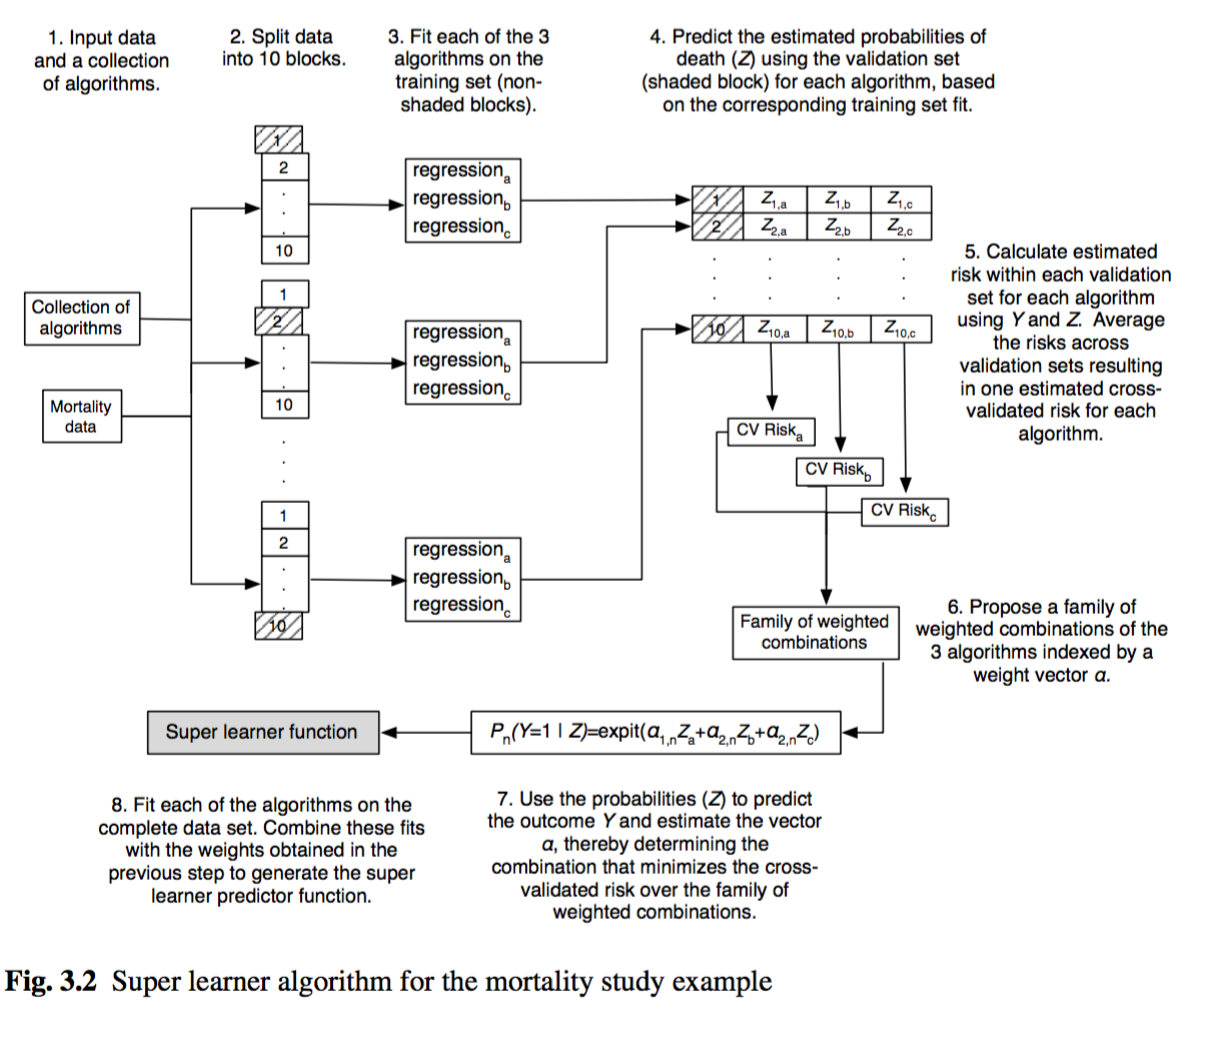
\includegraphics[scale=0.45]{../paper/figs/SuperLearn2.png}
		\end{center}
\end{frame}

\subsection{Cross-Validated AUC}

\begin{frame}[fragile]
  	\frametitle{cvAUC -- an R package for....}
 		confidence intervals...
		AUC estimates with Super Learner
		what else did we do with this?
\end{frame}

\subsection{LASSO Regression}

\begin{frame}[fragile]
  	\frametitle{LASSO for Pairwise Gene Selection}
 		Regularized regression... \\
		What did we do here?
\end{frame}

\section{Results}
\subsection{Differential Expression in Exposures}

\begin{frame}[fragile]
  	\frametitle{Differential Expression --- Benzene}
 		\begin{table}[ht]
		\caption {Benzene} \label{tab:benzene} 
		\centering
		\begin{tabular}{rlrrr}
  			\hline
 			Gene & Ratio & P-value & Q-value \\ 
  			\hline
			ACSL1 & 1.86 & 0.00 & 0.00 \\ 
  			AQP9 & 2.44 & 0.00 & 0.00 \\ 
  			CLEC5A & 2.39 & 0.00 & 0.00 \\ 
  			IFNB1 & 3.06 & 0.00 & 0.00 \\ 
  			NFKB1 & 1.64 & 0.00 & 0.00 \\ 
  			PRG2 & 1.67 & 0.01 & 0.02 \\ 
   			\hline
		\end{tabular}
		\end{table}
\end{frame}

\begin{frame}[fragile]
  	\frametitle{Differential Expression --- Nickel}
 		\begin{table}[ht]
		\caption {Nickel} \label{tab:nickel} 
		\centering
		\begin{tabular}{rrrrrrr}
 			\hline
 			& logFC & AveExpr & t & P.Value & adj.P.Val & B \\ 
  			\hline
			NFKB1 & 1.11 & 9.65 & 5.63 & 0.00 & 0.00 & 3.00 \\ 
  			ACSL1 & 0.88 & 9.47 & 4.92 & 0.00 & 0.00 & 1.49 \\ 
  			PRG2 & -0.48 & 5.32 & -4.42 & 0.00 & 0.00 & 0.41 \\ 
  			IFNB1 & -0.41 & 3.83 & -3.93 & 0.00 & 0.00 & -0.65 \\ 
  			AQP9 & 1.02 & 9.53 & 3.70 & 0.00 & 0.00 & -1.16 \\ 
  			CLEC5A & -0.11 & 5.88 & -0.85 & 0.40 & 0.47 & -6.04 \\ 
  			 \hline
		\end{tabular}
		\end{table}
\end{frame}

\begin{frame}[fragile]
  	\frametitle{Differential Expression --- Smoking}
 		\begin{table}[ht]
		\caption {Smoking} \label{tab:smoking} 
		\centering
		\begin{tabular}{rrrrrrr}
 		 	\hline
 			& logFC & AveExpr & t & P.Value & adj.P.Val & B \\ 
 			 \hline
			PRG2 & 0.12 & 4.49 & 1.04 & 0.31 & 1.00 & -4.63 \\ 
  			AQP9 & 0.18 & 7.56 & 0.62 & 0.54 & 1.00 & -4.75 \\ 
  			NFKB1 & 0.14 & 8.01 & 0.61 & 0.54 & 1.00 & -4.76 \\ 
  			ACSL1 & -0.27 & 6.71 & -0.58 & 0.56 & 1.00 & -4.76 \\ 
  			CLEC5A & -0.12 & 4.43 & -0.52 & 0.61 & 1.00 & -4.78 \\ 
  			IFNB1 & -0.02 & 4.49 & -0.13 & 0.90 & 1.00 & -4.82 \\ 
  			\hline
		\end{tabular}
		\end{table}
\end{frame}

\subsection{Pairwise Gene AUC Estimates}

\begin{frame}[fragile]
  	\frametitle{StuffB}
 		\begin{table}[h]
		\caption{AUC estimates via Super Learner} \label{tab:auc}
		\begin{center}
		\tabcolsep=0.11cm
		\scalebox{0.7}{
		\begin{tabular}{rlllllll}
  			\hline
 			& Benzene & Nickel & PAD & Smoking & Arsenic & Stress & Arthritis \\ 
 		 	\hline
			ACSL1 \& AQP9 & 0.9113095 & 0.75 & 0.5935673 & 0.5307692 & 0.1785714 & 				0.3397516 & 0.2944444 \\ 
  			NFKB1 \& IFNB1 & 0.939881 & 0.85 & 0.2251462 & 0.2653846 & 0.3285714 & 				0.3847826 & 0.437037 \\ 
  			PRG2 \& ACSL1 & 0.9204762 & 0.9 & 0.7339181 & 0.6615385 & 0.4666667 & 					0.3745342 & 0.3555556 \\ 
  			PRG2 \& CLEC5A & 0.9382143 & 1 & 0.5204678 & 0.6846154 & 0.5 & 0.3888199 & 			0.7148148 \\ 
  			NFKB1 \& CLEC5A & 0.9057143 & 0.8625 & 0.2704678 & 0.5769231 & 0.2428571 & 			0.2664596 & 0.6740741 \\ 
  			ACSL1 \& CLEC5A & 0.9150595 & 0.8375 & 0.6842105 & 0.6923077 & 0.15 & 					0.3409938 & 0.6703704 \\ 
   			\hline
		\end{tabular}
		}
		\end{center}
		\end{table} 
		\small stuff
\end{frame}

\section{Conclusions}

\subsection{So What?}

\begin{frame}[fragile]
  	\frametitle{Why Should Anyone Care?}
 		what is science? \\
		what is statistics?
\end{frame}

\begin{frame}[fragile]
  	\frametitle{(Bio)Statistics Saves Lives!}
 		what is science? \\
		what is statistics?
\end{frame}

\subsection{Going Forward}

\begin{frame}[fragile]
  	\frametitle{If We Could Do It All Again...}
		what is science? \\
		what is statistics?
\end{frame}


\end{document}
